\documentclass[english]{textolivre}

% metadata
\journalname{Texto Livre}
\thevolume{18}
%\thenumber{1} % old template
\theyear{2025}
\receiveddate{\DTMdisplaydate{2024}{3}{21}{-1}}
\accepteddate{\DTMdisplaydate{2024}{6}{22}{-1}}
\publisheddate{\DTMdisplaydate{2025}{1}{22}{-1}}
\corrauthor{Edurne Goñi Alsúa}
\articledoi{10.1590/1983-3652.2025.51717}
%\articleid{NNNN} % if the article ID is not the last 5 numbers of its DOI, provide it using \articleid{} commmand 
% list of available sesscions in the journal: articles, dossier, reports, essays, reviews, interviews, editorial
\articlesessionname{articles}
\runningauthor{Goñi-Alsúa y Rejas Vicente}
%\editorname{Leonardo Araújo} % old template
\sectioneditorname{Daniervelin Pereira}
\layouteditorname{João Mesquita}

\title{Educational methodologies and didactic audiovisual translation: Results of an implementation of combined revoicing and subtitling in a class of primary education with the Montessori method}
\othertitle{Metodologias educacionais e tradução audiovisual didática: resultados de uma implementação de dublagem e legendagem combinadas em uma turma do Ensino Fundamental com o método Montessori}

\author[1]{Edurne Goñi-alsúa, ~\orcid{0000-0002-7488-2689}\thanks{Email: \href{Edurne.goni@unavarra.es}{Edurne.goni@u navarra.es}}}\affil[1]{Universidad Pública de Navarra, Pamplona, Spain.}
\author[1]{Galder Rejas Vicente~\orcid{0009-0007-4495-100X}\thanks{Email: \href{rejas.132134@e.unavarra.es}{rejas.132134@e.unavarra.es}}}


\addbibresource{article.bib}

\begin{document}
\maketitle
\begin{polyabstract}
\begin{english}
  \begin{abstract}
      Among the new methodologies developed to teach the L2, Didactic Audiovisual Translation (DAT) has proven to be highly successful as it deals with the four skills in a multimodal environment, which appears to increase motivation. This paper presents the results of a DAT implementation in an Elementary classroom (11-to-12-year-old children) in a school which follows the Montessori Method. Twenty-four children, divided into groups of four, chose their favourite scenes from the TV series \emph{Goenkale} (broadcast on the Basque channel Euskal Televista 1) and translated, dubbed and subtitled them from their L1, Basque, into the L2, English, by means of the tool VideoPad. As Montessori Pedagogy does not include tests, the authors could not follow the experimental scheme of pre and post-test to observe any improvement in language acquisition. Data was therefore collected by the teacher, and subsequently analysed considering the mistakes made by the pupils during the process.  Pupils additionally completed a questionnaire, which indicated high levels of satisfaction towards this approach, thereby opening a new didactic path within Montessori Methodology. 

    \keywords{Didactic Audiovisual Translation (DAT) \sep Montessori Method \sep Dubbing \sep Subtitling \sep Primary Education}
  \end{abstract}
\end{english}

\begin{portuguese}
\begin{abstract}
    Dentre as novas metodologias desenvolvidas para o ensino de L2, a Tradução Didática Audiovisual (TDAV) tem-se revelado de grande relevância, uma vez que faz convergir as quatro competências num ambiente multimodal, o que motiva os alunos. Neste artigo apresentaremos os resultados de uma implementação baseada nesta metodologia, realizada numa turma do 6º ano do ensino básico (11 a 12 anos de idade), numa escola do método Montessori. Os vinte e quatro alunos, divididos em grupos de quatro, escolheram as suas cenas preferidas da série televisiva \emph{Goenkale} (da \emph{Euskal Televista 1}) e desenvolveram uma unidade didática na qual traduziram, dublaram e legendaram indiretamente (basco L1 para inglês L2) utilizando o programa VideoPad. Como a pedagogia Montessori não inclui testes, não foi possível desenvolver o esquema experimental de pré e pós-teste, mas o professor pôde recolher os erros cometidos para os incluir em unidades didáticas posteriores. Outro aspeto positivo foi a resposta dos alunos nos questionários de satisfação, que mostraram resultados favoráveis, abrindo novas vias didáticas na pedagogia Montessori.  

\keywords{Tradução audiovisual educacional \sep Pedagogia Montessoriana \sep Dublagem \sep Legendagem \sep Educação primária}
\end{abstract}
\end{portuguese}

% \begin{spanish}
% \begin{abstract}
%   Entre las nuevas metodologías desarrolladas para la enseñanza de la L2, la Traducción Audiovisual Didáctica (TAD) ha demostrado que es de gran relevancia, ya que en ella convergen las cuatro habilidades en un entorno multimodal, lo que motiva a los estudiantes. En este artículo vamos a presentar los resultados de una implementación basada en esta metodología, llevada a cabo en una clase de 6º curso de educación primaria (12-13 años de edad) en un colegio del método Montessori. Los veinticuatro alumnos, divididos en grupos de cuatro, eligieron sus escenas favoritas de la serie de televisión Goenkale (de Euskal Televista 1) y desarrollaron una unidad didáctica en las que tradujeron, doblaron y subtitularon de manera indirecta (L1 vasco a L2 inglés) por medio del programa VideoPad. Dado que la pedagogía Montessori no contempla la realización de tests, no se pudo desarrollar el esquema experimental de pre y post test, no obstante, el profesor pudo recoger los errores cometidos para darles cabida en unidades didácticas posteriores. Otro aspecto positivo fue la respuesta de los alumnos en los cuestionarios de satisfacción, que mostraron resultados favorables, lo que abre nuevos caminos didácticos en la pedagogía Montessori.  
% \keywords{Traducción Audiovisual Didáctica (TAD) \sep Pedagogía Montessori \sep Doblaje \sep Subtitulación \sep Educación primaria}
% \end{abstract}
% \end{spanish}

\end{polyabstract}

\section{Introductioon}\label{sec-introduction}

Event journalism mainly contemplates homicides, traffic accidents, drug
trafficking and robberies. Also, suicides, accidental falls, and
drowning, although the same informative treatment is not always applied
to all of them \cite{olivar2020tratamiento}.

Among all these topics, traffic accidents prevail in terms of
information compared to the rest due to their practically daily
frequency, the victims, and deaths they generate, the spectacularity and
visual impact of the images and the social alarm they arouse
\cite{rodriguez2011informacion}.

Event journalism understood until now as \enquote{specialized journalistic
information that deals with a varied subject centered on the commission
of crimes, accidents, catastrophes and curious and surprising facts}
\cite[p. 2]{rodriguez2011informacion}, faces in the 21st century the challenge
of a new technological dimension that allows the possibility of
producing news through automated journalism \cite{jamil2021automated}. In this
sense, people are already beginning to talk about \enquote{Robot Journalism},
\enquote{Automated Journalism} and even \enquote{Cognitive Journalism} where Artificial Intelligence (AI) has begun to occupy a field traditionally dominated by the human factor in the management of organizations. Also, in the media and in society through the application of Data Mining, to generate
algorithms that allow automation of management and refer it to the work
of bots in the production of news \cite{tunez2020from}.

It may seem that the journalistic profession is seemingly oblivious to
the robotization of newsrooms, but the origin of mass automation dates
to 2015, when the Associated Press (AP) automatically generated 3,000
\enquote{corporate earnings} stories in the US each quarter (IMT, 2019).

The editorial line, the agenda setting itself and the political
orientations of each communication media generate differences in the way
of covering the news about accidents \cite{arce2017accidentalidad}, but, within the information of events, it seems that the media
have shown a preference for certain types of news and events \cite{duran2020responsabilidad}. Specifically, it is expected to find a greater
number of news items referring to traffic accidents compared to other
types of events.

The agenda-setting theory maintains that the media influence the issues
that concern and speak about citizens, that is, that they can shape the
public agenda, in this case making it easier for citizens to talk
preferentially about traffic accidents over other types of events
\cite{scheufele2007framing}.

When the media publishes a greater amount of news about traffic
accidents, readers are not only informed about it, but they are also
influenced to think and give their opinion on that topic. In other
words, the media have a certain capacity to establish the agenda of the
set of issues about which a society speaks or is debated at a given
moment \cite{mccombs1972agenda}. In this way, it is intended to influence
the construction of news and information that they send to the public
\cite{vos2015how}.

It is also intended to obtain an answer on whether this greater number
of news publications on traffic accidents responds to a rigorous
elaboration and with its own elaboration or if the media are limited to
automatically transferring the information, they receive from the
emergency services. The media are in permanent contact with these
services, which are the ones who send them the necessary information to
produce news about traffic accidents, but the immediacy and permanent
updating of this information affects their journalistic rigor,
especially in digital newspapers.

According to González Ortiz, head of the \enquote{events and courts section} of
\emph{Diario de Navarra}, the main sources are the emergency services
and the police (personal communication, October 24, 2018). Crime
reporters draw on a variety of sources including:
\begin{itemize}
	
\item The police (through their press offices);
\item News agencies (mainly from \emph{EFE} and \emph{Europa Press});
\item Those of authors, victims, and witnesses (important sources but
difficult to obtain);
\item The judicial ones (the event journalist is usually also a court
journalist);
\item Undetermined sources (with and without attribution);
\item Other sources (forensic, penitentiary, neighborhood, union, health,
state, regional or municipal administrations, the media or traffic,
surveillance, emergency, or relief services \cite{rodriguez2015manual}.
\end{itemize}

Among all of them, journalists resort more frequently as a source of
information to prepare news about events to the police sources, which
include the National Police Corps, Local Police and Civil Guard, which
are the ones that make up the Security Forces and Corps of the State, as
established in Organic Law 2/1986, Security Forces and Corps (1986).
There are also specific services in each autonomous community.

The general objective of this study is to analyze the similarities
between news about traffic accidents (headlines and complete
journalistic pieces) published in different digital media.

The following are proposed as specific objectives:

Obtain information about the existence and repetition of exact news of
traffic accidents.

Obtain enough evidence to conclude that the media carry out a simple
dump of the news obtained from the emergency services and that,
therefore, there is an automated journalism model for the transmission
of news about traffic accidents.
\section{Theoretical Framework}\label{sec-theoreticalframework}

\subsection{Audio visual Translation and Didactic Audio visual Translation} \label{sub-sec-audiovisualtranslation}

As posited by \textcite{diaz-cintas2012subtitulos}, audio-visual translation (AVT) can be
defined as the process of transferring the cultural and linguistic
content of an audio-visual medium into another language. In doing so, it
is essential to consider the restrictions inherent to the medium in
question and to respect the original communicative purpose. Prior to
this definition, \textcite{diaz-cintas2009new} expounded that AVT had become a
crucial means of disseminating audio-visual content, not only on an
international scale, but also to ensure the accessibility of multimodal
content to diverse audiences.

The three principal modes of AVT are subtitling, dubbing and audio
description. In their study, \textcite{talavan2023didactic} define subtitling as the translation of a dialogue
into written form, text which is then placed at the base of the screen.
Moreover, dubbing entails the replacement of the original dialogue with
that in the target language, ensuring that the translated audio
syncronises with the movements of the actors' lips. As
a final point, audio description aims "to make the visual content of an
event accessible by conveying it into spoken words" \cite[p. 246]{ibanez2016audiodescription}.

Conversely, \textcite{talavan2019traduccion} defines Didactic audiovisual translation
(DAT) as the didactic application of AVT procedures to the teaching of
the L2. This researcher posits that DAT has its roots in the 1980s, when
researchers and scholars began to recognise the potential of this
approach to language teaching and started to incorporate subtitles as a
tool in language laboratories. Furthermore, \textcite{fernandez-costales2023tradilex} add that students must utilise technology (new tools
available on the internet) and employ the specific strategies associated
with each mode.

As early as 2009, \citefirstlastauthor{diaz-cintas2009new} emphasised the significance of DAT in L2
instruction, noting that it enables learners to engage with native
speakers' productions, thereby facilitating a more
genuine encounter with the L2 and its associated culture. In this way,
DAT has demonstrated to be an effective tool, as it engages learners by
providing them with authentic audio-visual materials, which allows to
immerse themselves not only in the language, but also in the target
culture. \textcite{fernandez-costeles2021} concurs with this assertion, having
conducted research into the effects of DAT on the learning of the L2 in
a primary education environment.

Additionally, \textcite{chaume2018audiovisual} emphasised that this approach facilitates a
more profound comprehension of the L2 through the combination of
auditory and visual input, thereby enabling learners to discern the
authentic, natural usage of language by native speakers. In this regard,
\textcite{gonzalez-vera2016audiovisual} illustrate that DAT facilitates more
effective learning by offering immediate feedback on pronunciation and
grammar, promoting more rapid language development.

\subsection{Didactic Dubbing and Subtitling}\label{sub-sec-didacticdubbing}

The combination of didactic dubbing and subtitling facilitates the
integration of the four linguistic skills. The primary focus of dubbing
is on oral skills, namely listening comprehension and speaking, whereas
subtitling is more closely aligned with written skills, namely reading
comprehension and writing. In addition to the aforementioned skills, we
can include the fifth skill, translation \cite{Carreres03072017}.

Regarding dubbing, \textcite{diaz-cintas2012subtitulos} mentions that students benefit
from exposure to a diverse range of dialects and accents. Furthermore,
it capacitates learners to enhance their oral comprehension and speaking
abilities concurrently, while fostering motivation through the
incorporation of a multimodal component. Moreover, it facilitates the
acquisition of the L2 in an authentic and natural manner
\cite{fernandez-costales2023tradilex}, as students engage with
genuine oral language in authentic contexts, diverging from the
structured materials typically provided in textbooks.

The benefits of subtitling have also been the subject of academic
investigation. \textcite{ÁlvarezSánchez_2017} asserts that the utilisation of
subtitles not only fosters the development of linguistic skills but also
upgrades the comprehension of paralinguistic and cultural elements. It
also encourages self- and cooperative learning, with learners at the
core of the learning process. Likewise, she explains that audiovisual
media reflects a multitude of communicative scenarios, thus facilitating
comprehension of an oral language text through the utilisation of
non-linguistic elements. Adding to this, \textcite{lertola2018translation} elucidates that
the advantages of employing subtitling are analogous to those of
translation. However, there is an additional benefit, as learners are
not merely translating a text from the source language to the target
language; they are also exposed to audiovisual material, which enables
them to observe and listen to authentic communication scenarios.
Additionally, \textcite{soler2020} states that subtitling enhances
vocabulary acquisition, provides motivation, facilitates productive
abilities (specifically, speaking and writing), ameliorates the L1, and
strengthens attention skills. As will be demonstrated, these
characteristics are consistent with the communicative approach that is
intended in Spanish L2 curricula.

Two previous studies have examined the combination of dubbing and
subtitling in L2 classes. \textcite{talavan2015first} put forth an
implementation of reverse subtitling and dubbing with the objective of
"improving oral and written production skills, along with general
translation competence" \cite[p. 169]{talavan2015first}. Their approach yielded highly
promising outcomes in terms of language acquisition. Similarly,
\textcite{BELTRAMELLO_2019} conducted an in-class implementation in accordance
with the aforementioned parameters. In her conclusions, she states that
the combination of the two modes is effective because, in addition to
facilitating language acquisition, students are exposed to "pragmatic
phenomena" \cite[p. 106]{BELTRAMELLO_2019}. In the process of dubbing, learners are required to
direct their attention towards the objectives of the speaker and the
utilisation of specific expressions, rather than others. Furthermore,
students have the opportunity to practise pronunciation, intonation, and
some paralinguistic aspects of language, thereby improving their
fluency. According to this scholar, ``it seems to reveal an untapped
potential in the combination of subtitling and revoicing as an aid to
language learning that offers abundant possibilities to practice and
develop different areas of language competence, such as pragmatic
competence'' \cite[p. 6]{BELTRAMELLO_2019}.

In light of the above, it can be posited that working with both DAT
modes concurrently represents an effective pedagogical approach. This
combination capacitates learners to simultaneously develop their
comprehension and production skills. Additionally, it improves
motivation, as students engage in a multimodal environment with
controlled exposure to authentic language usage in authentic contexts.

\subsection{The Montessori Method}\label{sub-sec-themontessorimethod}

The aim of developing innovative pedagogical approaches that align with
the needs of learners can be traced back to the 19th century. In
conjunction with the advent of new psychological theories, scholars
understood the necessity for a more individualised approach to teaching,
with a focus on the needs of the learner. Among the approaches that
emerged in this context were the Montessori Method or the Scientific
Pedagogy method, which was based on Maria Montessori\textquotesingle s
observations that children were capable of learning independently,
without the direct supervision of adults \cite{pla2007}.

\textcite{lillard2013playful} points that the Montessori Method is an educational
approach with the aim of promoting the holistic development of the
child. Its fundamental premise is the belief that children are innately
inclined towards learning. Consequently, educators must establish an
engaging and nurturing setting, provide individualized guidance through
experiential learning opportunities and encourage self-directed learning
by means of a blend of autonomy, suitable educational resources and
self-discipline \cite{marshall2017montessori}. Moreover, \textcite{pla2007}
assert that this method is founded upon four principal tenets: preparing
children for life, fostering a conducive learning environment,
refraining from undue interference in the learning process, and
providing sensorial materials to improve sensory development.

In addition, \textcite{marshall2017montessori} maintains that this method relies on the
development of two essential components: emotional and social skills.
The first seeks to ameliorate the emotional skills that help children
cope with the challenges of everyday life. The second focuses on
cooperation, empathy and mutual respect among students, and is performed
by activities which require cooperation. This way, learners build
relationships with their peers.

\textcite{montessori1937metodo} challenged the prevailing pedagogical trends of the
time, advocating for a teaching approach that empowers children to learn
through independent action. She emphasised the importance of educators
obtaining precise and logical observations of children, which serve as
the foundation for their instructional decisions. Accordingly, the
pedagogical approach is founded upon exploration and discovery, wherein
pupils progress within a tranquil, respectful, and structured milieu
with the objective of fostering autonomy. This signifies a shift in the
role of the teacher, moving from a director who oversees both
children\textquotesingle s learning and behaviour \cite{denervaud2019} to a supportive figure who establishes a
nurturing environment, in which pupils are able to flourish and reach
their full potential \cite{marshall2017montessori}. Pupils are encouraged to work
independently at their own pace in an environment replete with tangible
materials designed to promote discovery, exploration, and, most
crucially, creativity \cite{marshall2017montessori}. \textcite{denervaud2019} emphasise the necessity for these materials to be
self-correcting, thus enabling children to learn through trial and
error.

Additionally, \textcite{pla2007} claim that it is imperative
to respect the rhythms of pupil growth, requiring that teachers adapt
the content and devise individualised plans in accordance with the pace
of each child. Moreover, the aforementioned plans must be aligned with
the child\textquotesingle s interests, while also fostering
self-discipline. Furthermore, the learning proposals must develop five
key aspects: practice, imitation, repetition, classification and order.

It is therefore necessary to implement changes to the layout of the
classes and the grouping of the pupils. In the first case, \textcite{pla2007} explain that the classrooms must be reorganised, with the
elimination of desks, banks and class platforms for teachers, and the
adaptation of furniture to the height and strength of children. This
signifies that the classrooms are constituted as a structured framework,
which facilitates access to the materials and delineates specific spaces
to play, speak, rest and listen. Secondly, \cite{lillard2013playful} points that
pupils should be distributed in mixed-age classrooms, separated by a
range of three years: infants to three-year-olds, three to
six-year-olds, six to nine-year-olds, and from nine to twelve-year-olds.

This approach is founded upon the premise that children learn through
active engagement \cite{pla2007}. Consequently, didactic
workshops represent an efficacious instrument for the organisation of
educational activities. Among the advantages is the fact that workshops
facilitate hands-on teaching, which helps to maintain
students' interest and attention. Moreover, workshops
can be tailored to the specific abilities and requirements of each
pupil, thereby optimising the learning process. Additionally, workshops
facilitate teamwork and creativity, as children can engage in
collaborative activities. Nowadays, these learning environments have
evolved to encompass both physical spaces, such as science laboratories
or kitchens, and virtual environments. Nevertheless, the underlying
rationale remains consistent: learners engage in experiential learning
activities to apply the concepts they have acquired, thereby developing
the practical skills they will require in their future endeavours.

Moreover, this approach places an emphasis on the cultivation of
critical thinking abilities throughout the learning process \cite{murray2011montessori}. Pupils are encouraged to engage in exploration, discovery and
questioning to gain a deeper understanding of their surrounding
environment, which provides numerous opportunities for mutual assistance
\cite{pla2007}. The efficacy of this approach has been the
subject of considerable investigation, with \cite{lillard2013playful} demonstrating
its advantages in domains such as cognitive development, academic
achievement and self-discipline.

Some of the objectives of this approach are aligned with those of DAT.
On the one hand, both are based on the development of
students' thinking skills. According to \textcite[p. 214]{ghaffari2017montessori}, "the process of independent
problem solving creates self-confidence and critical thinking skills".
Translation is categorized alongside the highest order thinking skills,
according to Bloom's Taxonomy. Conversely, both methods
encourage collaborative work, as the majority of DAT activities are
conducted in pairs or groups. Lastly, both methods facilitate
learners' autonomy in learning, allowing them to work
at their own pace while the teacher serves as a guide, providing access
to learning resources.

\subsection{Spanish Legislation on Education and DAT}\label{sub-sec-spanishlegislationoneducationanddat}

The latest Law on Education \cite{lomloe2020} and the Organic Law on the
Foral Decree 67/2022 of the Foral Community of Navarre establish the
compulsory curriculum for all schools in the region. With some additions
due to the particularities of the Community, the latter specifies what
the former decrees.

In regard to the teaching of the L2, it is asserted that the focus
should be on the development of oral skills, with educators providing a
range of tools to facilitate student engagement with the content.
Moreover, educators must promote instrumental learning, which enables
learners to develop other competencies and meaningful learning, by
integrating the different competences in the execution of projects, so
that students solve problems cooperatively, what strengthens autonomy,
reflection and responsibility. Additionally, the L1 will be employed
solely as a support tool in the acquisition of the L2. Finally, learners
must allocate time on a daily basis to audio-visual communication and
the promotion of creativity and scientific inquiry.

The legislation requires educators to provide multiple tools to
encourage learner engagement. The world in which students live is
multimodal. Video clips, online games, films and TV series constitute
the majority of their leisure activities. It could therefore be assumed
that introducing these new languages into the classroom will make
learners feel more at ease, which will in turn improve their motivation
and, consequently, the acquisition of the L2.

Undoubtedly, DAT promotes instrumental learning as students work with a
variety of inputs, including text, audio and the cultural contexts of
multimodal texts, and have to manipulate the language in order to align
it with the image. In addition, it strengthens autonomy and reflection,
as learners can work independently or in collaboration with others,
which encourages them to problem-solve collectively and improves their
sense of responsibility. Finally, it integrates a range of competencies,
including linguistic communication, plurilingualism, digital
proficiency, personal and social skills, the capacity to autonomous
learning, consciousness, and cultural expressions \cite{Bobadilla-Pérez_CarballodeSantiago_2022,rodríguez-Arancón2023}, thereby implying
life-long learning, which is a fundamental aspect of the current
teaching and learning process.

Although the current legislation does not contemplate the use of the L1
and of translation in the class, \textcite{Carreres03072017,Colina03072017} have suggested that
translation should be considered as the `fifth skill', which ``can be
used as a pedagogical tool to integrate the original four skills to
enhance second language study'' \cite[p.~2]{Colina03072017}.

\section{Proposal}\label{sec-proposal}

The research conducted was driven by two main questions, intended to
complement existing studies, and to gain insights into two key areas:
the first refers to the teaching-learning aspect, and the second to the
enjoyment of the pupils.

\begin{itemize}
    \item Does the implementation of a DAT didactic unit, based on the
    combination of interlingual indirect subtitling and dubbing (L1 Basque)
    enhance the results on acquisition of English language?

    \item Is DAT a motivational method for students of primary education
    following alternative schooling methodologies?
\end{itemize}

\subsection{Participants}\label{sub-sec-participants}

This implementation was conducted in a primary education school situated
in a middle-class neighbourhood of Pamplona, Spain, which follows the
Montessori Method, whose L1 is Basque. While not all pupils who
participated in this research speak this language at home, all classes
are taught in Basque. In the area, there is another school with two
lines of L1, Basque and Spanish, and a high school with the same L1
paradigm.

This school is committed to an active approach to learning, utilising
Montessori-inspired materials and a class structure that incorporates
learning environments and project-based learning as the primary
pedagogical methodology. The aforementioned pedagogical approach is
employed with the objective of fostering the development of
self-regulation and autonomy in students, as well as enhancing their
capacity for collaborative work through the utilisation of flexible
group structures and other active educational resources.

A total of 24 pupils, comprising the 6th course of primary education and
aged between 11 and 12 years old, participated in the project. The
pupils were divided into groups of four and worked together throughout
the implementation period. The participants demonstrated a level of
English proficiency corresponding to A1, as defined by the Common
European Framework of Reference for Languages (CEFR). Parents were
informed and gave their consent to the project, which has been approved
by the corresponding committee of UPNA.

\subsection{Materials}\label{sub-sec-materials}

During the implementation, learners were provided with the scripts of
the scenes and employed the class computers, dictionaries (both physical
and online), voice recorders and the editing app VideoPad
(\url{https://www.nchsoftware.com/videopad/es/index.html}). Finally, the
pupils completed a questionnaire (\Cref{annex-01}) to ascertain their level of
satisfaction with the implementation process, allowing for both
quantitative and qualitative results to be gathered.

\subsection{Design}\label{sub-sec-design}

One of the distinctive characteristics of the Montessori approach is the
absence of conventional testing and examination procedures.
Consequently, the implementation did not adhere to the customary
experimental pre-test--post-test design. Nevertheless, the instructor
could delineate certain guidelines to enhance the acquisition of the L2,
based on the errors that students had committed throughout the sessions.

A further aspect of this approach is that learners must be free to
select their own areas of interest and determine their own learning
strategies. This is reflected in the fact that they spent two sessions
searching for a TV series and a particular scene that they wished to
translate, dub and subtitle. As this was the first time that such a
project was implemented in the school, the instructor elected to develop
it in the Kitchen Corner, the designated workspace intended for the
duration of the internship.

The initial proposal was to implement a didactic unit on subtitling.
However, the instructor determined that pupils could undertake a
combined project encompassing both dubbing and subtitling, given the
absence of time constraints typically encountered in traditional
educational settings. This alteration has furnished the implementation
with an unanticipated degree of depth. As a result of this expansion,
the final products created by the students were the selected scenes
translated from the L1 to the L2, and both dubbed and subtitled. The
project was developed over four days, in sessions of 45 minutes each.
The subsequent schema was followed:

\begin{itemize}
    \item Choice of TV series and scene: two sessions
    
    \item Transcription and translation of the script: two sessions
    
    \item Audio recording: three sessions
    
    \item Scene editing: three sessions
\end{itemize}

\subsection{Procedure}\label{sub-sec-procedure}

\subsubsection{Day 1. The choice of series and scenes}

The session commenced with the activation of prior knowledge through the
posing of questions to the pupils, such as "What are your favourite TV
series?" This enabled the teacher to ascertain the
learners\textquotesingle{} interests, thereby facilitating the
personalisation of the learning process in accordance with their
preferences. A further crucial element of these two sessions was the
formation of flexible groups, comprising learners with diverse
abilities, so that they could learn from one another. The pupils elected
to work with their preferred scenes from the television series
\emph{Goenkale}, which features teenagers and is set in the Basque
Country. It is broadcast on \emph{Euskal Telebista} 1 (ETB1). This is a
highly popular programme with a particularly strong viewership among the
adolescent demographic. Prior to the DAT practice session, the children
were required to imitate both the intonation and rhythm of the speech of
the character they were to dub.

\subsubsection{Day 2. Transcriptions and translations}

The first session comprised an examination of the scene and an endeavour
to identify a suitable transcription. The pupils were initially required
to view the scene on multiple occasions, with the objective of
facilitating an in-depth comprehension of the nuances embedded within
the dialogue. This approach was designed to facilitate a more
straightforward engagement with the language.

Following the viewing, the children conducted online research to find
the transcriptions of the dialogues, utilising a range of digital
platforms. In the event that the desired material was not accessible,
the pupils utilized YouTube, as it offers subtitles for a number of
videos. They then proceeded to transcribe the scene by manually copying
the subtitles.

In the second session, the children completed the transcription and
translated it from L1 to L2 using both physical and online dictionaries.
The instructor directed the students\textquotesingle{} attention to the
fact that language can convey double meanings and transmit cultural
expressions that, when translated literally, are devoid of meaning. The
teacher\textquotesingle s main role was to provide assistance. She
clarified doubts and illustrated the lexicon, ensuring that all learners
were able to comprehend the message conveyed in the script.

\subsubsection{Day 3. Audio recording}

In the initial session, the students engaged in practice activities,
which entailed reading the transcriptions in both languages and
commencing the recording of the L2 audio. In the subsequent sessions,
the children proceeded with the audio recording.

During the audio recording sessions, the pupils concentrated on
developing their pronunciation and fluency. As the teacher consistently
reiterated the importance of aligning the spoken text with the
corresponding mouth movements, the pupils undertook a process of review
and editing of their recordings, with the objective of ensuring that
they met the desired quality standards. In order to achieve this, it was
necessary for the children to consider the previous work, in order to be
able to adjust the text in the L2 to the rhythm of the original scene
and to align the audio with the video. In addition, pupils were required
to become proficient in the use of the VideoPad application in order to
gain familiarity with its various functions.

The final stage of the process involved the deletion of the audio from
the original scene and the insertion of the new audio files, which were
then adjusted to the rhythm of the scenes. The children proceeded to
implement the final modifications to their product. The instructor
offered feedback and guidance to assist the pupils in enhancing their
productive oral skills.

\subsubsection{Day 4. Scene subtitling and editing}

In the initial session, the pupils were instructed in the techniques of
video editing and were given the opportunity to improve their writing
skill as they worked on the subtitles. In the remaining two sessions,
the children continued subtitling to create the final product, which was
a scene that was both dubbed and subtitled. The software utilized by the
pupils was once more VideoPad, which also facilitates the creation of
subtitles. By the conclusion of the sessions, children had produced
videos with high-quality audio and accurate subtitles.

\subsection{Assessment}\label{sub-sec-assesment}

Upon completion of the implementation phase, both the pupils and the
teacher conducted an assessment of the various projects using an
evaluation rubric (\Cref{annex-02}). Children were evaluated on five distinct
criteria: translation accuracy, coherence between the visual and
auditory content, adequate use of language and grammar, cultural
adaptation, and creativity and originality.

This assessment rubric was devised for use by both teachers and
learners. The teacher subsequently provided a more detailed assessment
in each category, including additional commentary on the areas that
require improvement and on those in which the pupils had demonstrated
proficiency.

\section{Results}\label{sec-results}

This section is divided into three main topics. First, we will discuss
the social media platforms and languages students use, along with the
objectives they pursue when making videos. Second, we will describe what
students do before and after making videos. Third, we will examine
students' perceptions of language learning through video-making.

\subsection{Social media platforms, languages, and objectives}\label{sub-sec-socialmediaplatforms}

In general, 46 people, or only 21.7\% of the participants of the overall
questionnaire, reported that they occasionally had been making videos in
a broad sense (including reels and stories on Instagram). We will centre
most of our results section on these participants.

Stories on Instagram and videos on YouTube were the most frequently
produced types of videos according to \Cref{fig-01}. Instagram stories are
used 28.3\% \emph{sometimes} and 13\% \emph{frequently}, meanwhile,
videos on YouTube are made 34.8\% \emph{sometimes} and 8.7\%
\emph{frequently}. Notably, almost nobody used Twitch and a small
percentage of the students made videos on TikTok (15.2\%).

\begin{figure}[htbp]
\centering
\begin{minipage}{\textwidth}
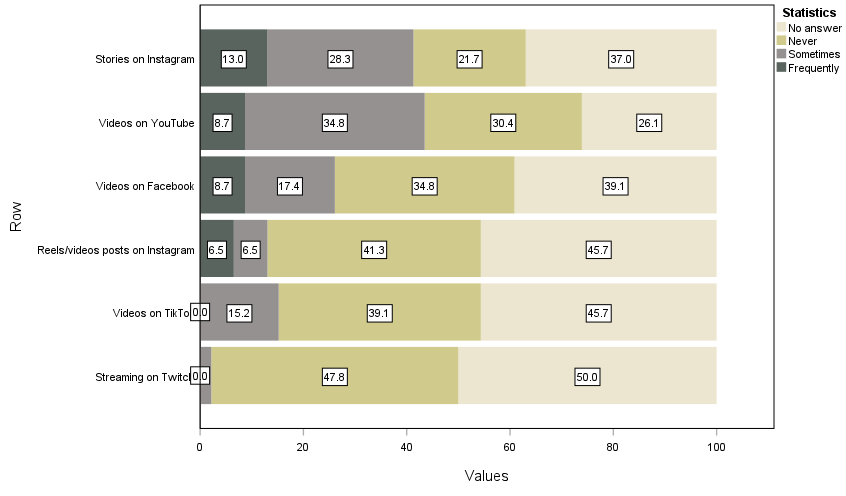
\includegraphics[width=\textwidth]{Fig-1.png}
\caption{Frequency of production of different types of videos.}
\label{fig-01}
\source{Own elaboration.}
\end{minipage}
\end{figure}

We also observe a pattern across all platforms, with the least common
response being to make videos frequently (from 13\% on Instagram to 0\%
on TikTok), indicating that a relatively low percentage of respondents
makes videos frequently, especially in comparison with the practice of
watching videos \cite{shafirova2023}. Moreover, we found a
correlation between the age of the students and the types of video
production. The correlation was found in the social media platforms of
TikTok, YouTube and Facebook, in which older students (older than 36)
tend to make videos for Facebook (due to cross tabulation with Pearson
chi-square test with 0.019 significance in case of YouTube and 0.004 in
case of Facebook). Meanwhile, younger students (from 18 to 23) tend to
make videos on TikTok (due to cross tabulation with Pearson chi-square
test with 0.008 significance). It is noteworthy that, on Instagram, we
did not find any correlation with age.

In general, in our data, age does not influence the frequency of making
videos, however, it points out that some social media platforms are more
frequently used by younger respondents and some by slightly older
respondents (similarly found in the dataset concerning the US population
from \textcite{ortizo-spina2019}). Moreover, the students post videos in
different languages, mostly in Portuguese and English (\Cref{tab-04}), while
other languages have a relatively smaller presence (max. 20\% with
Spanish on Facebook).

\begin{table}[htbp]
\centering
\begin{threeparttable}
\caption{Languages and platforms of video production: multiple choice response.}
\label{tab-04}
\begin{tabular}{*{11}{l}}
\toprule
Platforms & \multicolumn{2}{c}{YouTube} & \multicolumn{2}{c}{Facebook} &  \multicolumn{2}{c}{Instagram} & \multicolumn{2}{c}{TikTok} & \multicolumn{2}{c}{Twitch} \\
\midrule
Portuguese & 22 & 88\% & 13 & 86.7\% & 19 & 95\% & 5 & 71.4\% & 0 & 0\% \\
English    & 13 & 52\% & 6  & 40\%   & 9  & 45\% & 5 & 71.4\% & 1 & 50\% \\
Spanish    & 3  & 12\% & 3  & 20\%   & 1  & 5\%  & 0 & 0\%    & 0 & 0\% \\
Italian    & 2  & 8\%  & 2  & 13.3\% & 1  & 5\%  & 0 & 0\%    & 0 & 0\% \\
French     & 1  & 4\%  & 2  & 13.3\% & 0  & 0\%  & 0 & 0\%    & 0 & 0\% \\
Crioulo    & 0  & 0\%  & 0  & 0\%    & 1  & 5\%  & 0 & 0\%    & 0 & 0\% \\
Persian    & 0  & 0\%  & 1  & 6.7\%  & 0  & 0\%  & 0 & 0\%    & 0 & 0\% \\
Other      & 2  & 8\%  & 1  & 6.7\%  & 1  & 5\%  & 2 & 28.6\% & 1 & 50\% \\
\rule{0pt}{3ex}%
Total & 44 & 176\% & 28 & 186.7\% & 32 & 160\% & 12 & 171.4\% & 2 & 100\% \\
\bottomrule
\end{tabular}
\source{Own elaboration.}
\end{threeparttable}
\end{table}




In comparison, our previous study shows that video consumption on social
media and streaming platforms could be considered more diverse and
plurilingual. Even though English and Portuguese were still the most
popular languages, Spanish was used by roughly half of the participants
on streaming platforms such as Netflix and HBO. Additionally, such
languages as French, Italian, Korean or Japanese were also present, with
more than 10\% on various platforms \cite{shafirova2023}. There
could be various reasons for this difference in language variety in
video production and consumption. One possible explanation could be the
amount of resources available for watching videos in languages you do
not have a perfect command of, such as subtitles in different languages,
captions, scripts and more \cite{shafirova2023}.

Moreover, we asked the participants if they tended to use several
languages in one video. The participants responded with 26.1\% ``yes'',
with the main objective of reaching out to a vast audience (41.6\%), or
because of being multilingual (30\%).

\subsection{Why students make and post videos}

To understand students' intentions behind video production, we asked
about their objectives when making videos. According to \Cref{fig-02}, the
majority of the students make videos to ``have fun'' (63\%), which goes
along with previous research on video creation beyond the classroom
\cite{zhang2022}.

\begin{figure}[htbp]
\centering
\begin{minipage}{\textwidth}
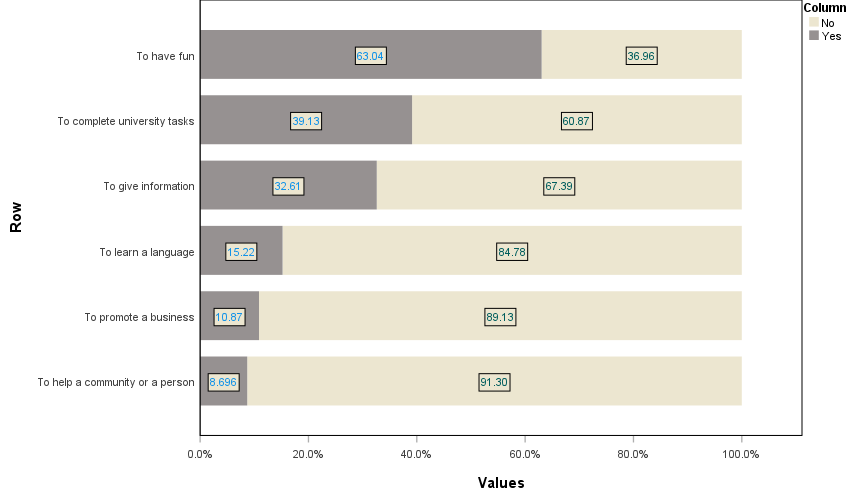
\includegraphics[width=\textwidth]{Fig-2.png}
\source{Own elaboration.}
\caption{Objectives to make videos.}
\label{fig-02}
\end{minipage}
\end{figure}

However, the second most popular answer is ``to complete university
tasks'' (39.1\%), which is a thought-provoking result indicating that
some of the university tasks require students to make videos (similar
results at the school level in \textcite{cassany2021}). It would be
valuable to explore the potential differences between the videos created
for leisure and those made as university tasks, even though these videos
would not necessarily be connected to language learning.

Moreover, the third answer was ``to give information'' (33\%), which
also seems like a serious and not entertaining goal, which can include
making videos or reposts of some news or events. This goes against the
assumption of some researchers that social media is always used only for
entertainment purposes \textcite{rosyida2019}. Also, the option ``to
learn a language'' was not popular (15.2\%), which is an expected result
as only 33\% of the participants are current language learners.

\subsection{What students do before and after producing videos}

Much like when watching videos online \cite{shafirova2023},
around half of the respondents were engaged in some communicative
actions before and after making a video. According to \Cref{tab-05} and \Cref{tab-06},
the communicative actions included searching (information or visuals),
reading (comments), writing (descriptions of the videos), watching
videos (to analyse similar videos), translating and interacting with
others (collaborating with others, responding to comments, making video
responses). The most frequent action before video production is
searching for information (\Cref{tab-05}), while the most frequent after
production is reading the comments or feedback on the videos (\Cref{tab-06}).
The options of writing descriptions or interacting with others were less
popular (roughly half of the responses).


\begin{table}[htbp]
\centering
\small
\begin{threeparttable}
\caption{Communicative actions made before video production.}
\label{tab-05}
\begin{tabular}{*{13}{l}}
\toprule
\multicolumn{1}{{>{\raggedright\arraybackslash}p{0.11\textwidth}}}{Actions} &
\multicolumn{2}{{>{\raggedright\arraybackslash}p{0.11\textwidth}}}{Search for information} &
\multicolumn{2}{{>{\raggedright\arraybackslash}p{0.11\textwidth}}}{Search for visual aid} &
\multicolumn{2}{{>{\raggedright\arraybackslash}p{0.11\textwidth}}}{Analyse similar videos} &
\multicolumn{2}{{>{\raggedright\arraybackslash}p{0.11\textwidth}}}{Write short descriptions} &
\multicolumn{2}{{>{\raggedright\arraybackslash}p{0.11\textwidth}}}{Collaborate with others} &
\multicolumn{2}{{>{\raggedright\arraybackslash}p{0.11\textwidth}}}{Make translations} \\
\midrule
Languages & N & \% & N & \% & N & \% & N & \% & N & \% & N & \% \\ 
Portuguese & 16 & 69.6\% & 11 & 47.8\% & 10 & 43.5\% & 11 & 47.8\% & 9  & 39.1\% & 7  & 30.4\% \\ 
English    & 18 & 78.3\% & 15 & 65.2\% & 11 & 47.8\% & 7  & 30.4\% & 7  & 30.4\% & 9  & 39.1\% \\ 
Spanish    & 3  & 13\%   & 2  & 8.7\%  & 3  & 13\%   & 1  & 4.3\%  & 2  & 8.7\%  & 1  & 4.3\%  \\ 
Italian    & 2  & 8.7\%  & 2  & 8.7\%  & 2  & 8.7\%  & 1  & 4.3\%  & 2  & 8.7\%  & 1  & 4.3\%  \\ 
French     & 2  & 8.7\%  & 2  & 8.7\%  & 2  & 8.7\%  & 0  & 0\%    & 2  & 8.7\%  & 1  & 4.3\%  \\ 
Chinese    & 1  & 4.3\%  & 1  & 4.3\%  & 0  & 0\%    & 1  & 4.3\%  & 0  & 0\%    & 0  & 0\%    \\ 
Persian    & 1  & 4.3\%  & 0  & 0\%    & 0  & 0\%    & 0  & 0\%    & 0  & 0\%    & 0  & 0\%    \\ 
Other      & 1  & 4.3\%  & 0  & 0\%    & 0  & 0\%    & 0  & 0\%    & 0  & 0\%    & 0  & 0\%    \\ 
\rule{0pt}{3ex}%
Total     & 44 & 191.2\% & 33 & 143.4\% & 28 & 121.7\% & 21 & 91.1\% & 22 & 95.6\% & 19 & 82.4\% \\ 
\bottomrule
\end{tabular}
\source{Own elaboration.}
\end{threeparttable}
\end{table}

Interestingly, if videos were mostly created in Portuguese and English,
the actions made before and after video production had more linguistic
variability, with the 7 languages present before video production, and
11 after production.

Furthermore, we made a comparison or cross-tabulation comparing the
participants\textquotesingle{} mother tongues with the actions taken
before video production (\Cref{tab-05}). The results showed that most
participants were using a foreign language before and after making a
video. In the case of activities made before video production, several
participants used such foreign languages as English, French and Italian.
Also, some participants used their mother tongues, including Portuguese,
Spanish, Chinese and Persian. Similar data emerged when comparing the
responses concerning the actions taken after posting the videos in
relation to the participants' mother tongues (\Cref{tab-06}).


\begin{table}[htbp]
\centering
\begin{threeparttable}
\caption{Communicative actions made after video production.}
\label{tab-06}
\begin{tabular}{*{7}{l}}
\toprule
Actions &
\multicolumn{2}{{{>{\raggedright\arraybackslash}p{0.25\textwidth}}}}{Read comments, chat, reactions} &
\multicolumn{2}{{>{\raggedright\arraybackslash}p{0.14285714285\textwidth}}}{Respond to the comments} &
\multicolumn{2}{{>{\raggedright\arraybackslash}p{0.14285714285\textwidth}}}{Make video responses to comments} \\
\midrule
Portuguese & 19 & 79.2\% & 8 & 33.3\% & 3 & 12.5\% \\ 
English    & 17 & 70.8\% & 9 & 37.5\% & 3 & 12.5\% \\ 
Spanish    & 7  & 29.2\% & 3 & 12.5\% & 1 & 4.2\%  \\ 
Italian    & 5  & 20.8\% & 3 & 12.5\% & 1 & 4.2\%  \\ 
French     & 5  & 20.8\% & 2 & 8.3\%  & 2 & 8.3\%  \\ 
Chinese    & 2  & 8.3\%  & 1 & 4.2\%  & 1 & 4.2\%  \\ 
Persian    & 2  & 8.3\%  & 1 & 4.2\%  & 2 & 8.3\%  \\ 
Russian    & 2  & 8.3\%  & 1 & 4.2\%  & 1 & 4.2\%  \\ 
Korean     & 1  & 4.2\%  & 1 & 4.2\%  & 1 & 4.2\%  \\ 
Crioulo    & 1  & 4.2\%  & 1 & 4.2\%  & 1 & 4.2\%  \\ 
Japanese   & 1  & 4.2\%  & 1 & 4.2\%  & 1 & 4.2\%  \\ 
Other      & 1  & 4.2\%  & 1 & 4.2\%  & 2 & 8.3\%  \\ 
Total      & 63 & 262.5\% & 32 & 133.5\% & 19 & 79.3\% \\ 
\bottomrule
\end{tabular}
\source{Own elaboration.}
\end{threeparttable}
\end{table}

For instance, in \Cref{tab-06}, most participants used English as a foreign
language when reading and responding to comments. Other foreign
languages included Spanish (only one respondent used it as a mother
tongue), French, Italian and Korean. These data indicate that students
engaged in communicative activities in foreign languages both before and
after making a video. This characterizes video production as interactive
and increases language input through various modes, including written,
oral, interactive, and information-seeking activities.

\subsection{The students' perceptions of language learning with video production and consumption}

The questionnaire included two questions about students' perceptions of
language learning while watching or producing videos. The questions went
as follows: ``To what extent do you agree with the statement:
Watching/producing videos in (an)other language(s) helped me in learning
this(ese) language(s)''.

In \Cref{fig-03}, we compare the answers to these questions divided into two
graphics (based on N-46), one focused on video viewing (blue) and the
other on video production (red). The line on video viewing is much more
accentuated in comparison with video production which has an almost
normal distribution.

\begin{figure}[htbp]
\centering
\begin{minipage}{\textwidth}
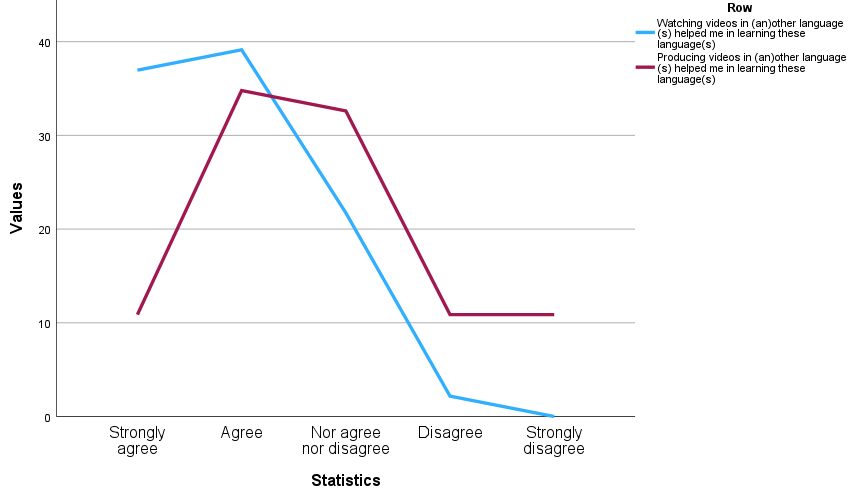
\includegraphics[width=\textwidth]{Fig-3.png}
\caption{Students' perceptions of language learning with the help
	of video watching/producing.}
\label{fig-03}
\source{Own elaboration.}
\end{minipage}
\end{figure}

It indicates that in the case of video watching, the students mostly
``strongly agree'' and ``agree'' (around 75\%) with the proposed
statement. However, in the case of video producing, most respondents
``agree'' or ``neither agree nor disagree'' (around 70\%), with some
respondents ``disagreeing'' and ``strongly disagreeing'' (around 22\%).
This comparison shows a division in opinions on the benefits of video
production, with more uncertainty in the results for video production
compared with video watching.

These results could be connected to the frequency of video production
compared to video viewing and the fact that students could be engaged in
very different forms of video production, from Instagram stories to
lengthy videos on YouTube. It can also be connected to our particular
dataset which includes students from non-language studies. In general,
we consider this discrepancy in data on video viewing and production an
interesting phenomenon for further investigation.

Additionally, we ran a cross-tabulation test with a Pearson Chi-Square
test to examine if there is a correlation between these students'
perceptions of video production (\Cref{fig-03}) and the fact that they are
current language learners (\Cref{tab-03}). The p-value (or significance) for
the Chi-Square test was 0.6, indicating no significant correlation
between these two variables. However, due to the small sample size,
seven cells had an expected count of less than 5, which may make the
results unreliable. To address this, we combined the cells ``agree'' and
``strongly agree,'' as well as ``disagree'' and ``strongly disagree,''
transforming the 5-level Likert scale into a 3-level scale. In this
adjusted analysis, only two cells had an expected count of less than 5,
making the results more reliable. Similar to the previous test, the
p-value was 0.3, indicating no significant correlation between these
categories. In addition, we ran the Fisher Exact test which is better
suited for smaller samples, nevertheless, it also did not indicate any
correlation ($p=0.7$ in the first case and $p=9.4$ in the second case).

These results indicate that there is no significant correlation between
these two categories. We also examined the categories of current
language learners and students\textquotesingle{} perceptions of video
watching, and similarly found no correlation (Chi-Square test, $p=0.5$;
Fisher Exact test, $p=0.7$). However, it would be beneficial to test this
hypothesis with a larger dataset to confirm these findings.

Moreover, we examined the relationship between the category of students'
perceptions of video production benefits and the departments where the
students study. We combined our categories into 1) Language Department,
2) Education and Psychology, and 3) Other to see if there are some
correlations between our specific dataset and the question. The
Chi-Square test showed no significant correlation $(p= 0.066)$, however,
the Fisher Exact test showed some significance $(p = 0.05)$. In this case,
as our dataset is small and 50\% of the results have an expected count
of less than 5, the Fisher Exact Test seems to be more reliable \cite{jung2014}.
\Cref{fig-04} also shows a strong indication of dependence between
these categories.

\begin{figure}[htbp]
\centering
\begin{minipage}{\textwidth}
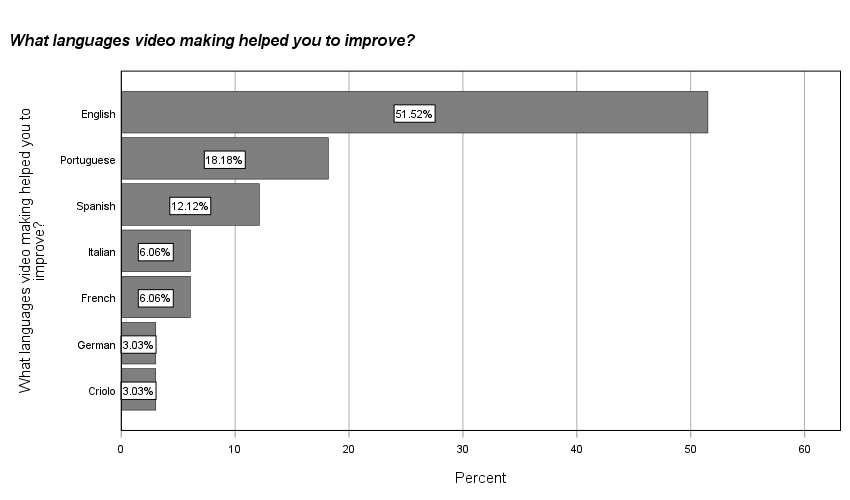
\includegraphics[width=\textwidth]{Fig-4.png}
\caption{Perceptions of the students on video production:
	department distribution.}
\label{fig-04}
\source{Own elaboration.}
\end{minipage}
\end{figure}

According to \Cref{fig-04}, we can see that in the Languages and Cultures
department, most students agree that video production helps in learning
a language (adjusted residual 1.6), while in Other Departments fewer
people agree with this statement (adjusted residual -2.5). In the
Department of Education and Psychology, fewer students disagreed that
video production could help language learning (adjusted residual -1.8).
The distribution observed here indicates more positive perceptions of
video production in the Department of Languages and Cultures. This
suggests that teaching methodologies in the Languages and Cultures and
the Education and Psychology departments may be influencing
students\textquotesingle{} perceptions. Additionally, when we tested the
correlation between a departmental distribution and students'
perceptions of video watching, we found no significant correlation using
either the Chi-Square test $(p=0.3)$ or the Fisher Exact test $(p=0.3)$.
Examining this question across different departments would be
beneficial, as our current dataset is too small to draw definitive
conclusions.

Moreover, 46\% of students chose the categories ``strongly agree'' and
``agree'' with the benefits of video production for language learning.
They also answered the next question regarding the languages that
video-making helped them learn (\Cref{tab-05}).

\begin{figure}[htbp]
\centering
\begin{minipage}{\textwidth}
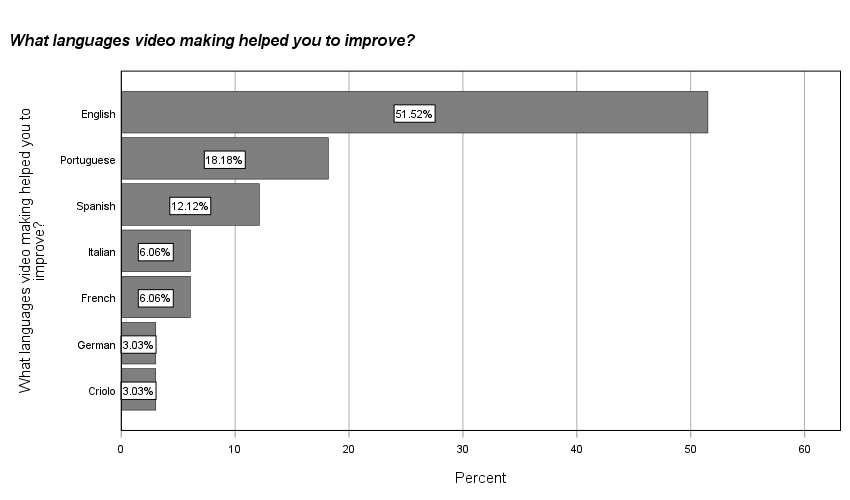
\includegraphics[width=\textwidth]{Fig-5.png}
\caption{Languages improved by making videos}
\label{fig-05}
\source{Own elaboration.}
\end{minipage}
\end{figure}

According to \Cref{fig-05}, the respondents chose a considerable variety of
languages, taking into account that only 21 people (from 46) responded
to that question and chose seven languages. English was the most popular
response, followed by Portuguese and Spanish. Notably, we can also see
\emph{Crioulo} derived from the Portuguese language (variation from Cabo
Verde) in the responses, which was completely absent from video viewing
responses \cite{shafirova2023}.

The students also responded to an open question concerning language
learning and video viewing/production: ``How have you improved your
language and cultural skills by watching/producing videos in different
languages?'' In the case of video viewing, we received 52 responses or
around 25\% of 212 respondents. According to our codebook (\Cref{annex-a}), 23
responses included the learning of vocabulary, oral comprehension had 9
responses, and pronunciation had 7. Students also noticed learning the
cultural aspects (7) of countries where languages are used and
underlined the importance of learning the language in the context of its
use (5). Overall, the detailed responses indicate that students view
this knowledge as important to share.

In the case of video production, we received 8 responses out of 46, in
other words, 17\% of the students responded, including such categories
as vocabulary (4), speaking (2) and cultural aspects (1). The answers
were less detailed than those in the viewing section, with a lower
overall response rate. Additionally, most responses came from the
Departments of Languages and Cultures and Education and Psychology. Some
responses highlighted that not only video production was beneficial for
language learning but also the work completed beforehand or afterwards
(\Cref{annex-a}). For instance, one respondent noticed: ``The research required
to produce most of my content has allowed me to widen my vision of the
English language and culture''.

We observe that students frequently highlighted vocabulary as the
primary area of improvement in both video viewing and production. This
suggests that, from the respondents\textquotesingle{} perspective,
vocabulary could be the most beneficial aspect of both practices.

\section{Discussion}\label{sec-discussion}
The analysis of participants' use and experience with
AI tools (R.Q.1) provides valuable insights into their engagement with
emerging technologies in both academic and non-academic domains. The
data reveals a diverse range of use patterns among participants,
showcasing a spectrum of preferences and approaches towards AI adoption.
While some participants actively employ AI tools for tasks such as idea
generation, translation, and language instruction, others exhibit a more
reserved attitude, either abstaining from their use entirely or
employing them sparingly. Moreover, participants display variability in
their choice of AI platforms, with preferences ranging from widely
recognized tools like Deepl and ChatGPT, as outlined by \textcite{schmidt2022} and to lesser-known options such as TWEE and Canva.
Notably, there is an evident openness among participants to explore new
AI technologies, as indicated by intentions to adopt novel tools and
experiment with additional functionalities of existing platforms.
Furthermore, participants frequently integrate multiple AI tools into
their workflow, combining different platforms to address various aspects
of academic tasks effectively. This integration underscores a holistic
approach to leveraging AI technologies, wherein participants draw upon
the strengths of each tool to optimize their productivity and outcomes.
Overall, the findings suggest that participants'
utilization and experience with AI are characterized by diversity,
variability, openness to exploration, integration of multiple tools, and
varied levels of experience. These insights provide a comprehensive
understanding of how participants engage with AI technologies to support
their academic and non-academic endeavors, emphasizing the multifaceted
nature of AI utilization in contemporary educational contexts.

These findings highlight the high familiarity and proficiency of
participants with AI for general purposes, which may translate into an
appreciation for its potential professional applications. As most
pre-service teachers belong to the digital-native generation, they are
likely to adapt easily to AI technology and recognize its potential for
future practice.

Concerning the R.Q.2, the results of the SWOT analysis are summarised in
\Cref{tab-02}. The internal analysis shows a clear representation of strengths
and weaknesses related to the nature of the app: participants report
practical uses of the resource for the teacher's perspective such as the
different activities, the speediness and usefulness of the software.
Regarding the weaknesses, they factor diversity, both in terms of
students with special needs (no option to adapt the activities within
the app) as well as language constrictions (only in English), while also
mentioning interface issues (e.g. video conversion). These findings
align with those by \textcite{ravshanovna2023}.

The results found on the external analysis of opportunities and threats
resonate to some extent with the answers for the internal analysis; this
can be explained by the fact that TWEE is an educational tool itself so
teachers analyse it as such. Therefore, the quick creation of diverse
and innovative activities is reported once again along with the
opportunities it provides for paying attention to students' likes, which
can be linked to the idea of personalised learning thanks to AI \cite{chen2020}. As far as threats and dangers, participants focus on the
detriments it may pose for students in terms of ethical concerns (e.g.
cheating) and learning factors (e.g. effort and attention span), while
the major concern for teachers would be to become superfluous.


\begin{table}[!htbp]
\centering
\caption{Results of the SWOT Analysis.}
\label{tab-02}
\begin{tabular}{ll}
\toprule
Strengths & Weaknesses\\
- Variety of resources & -Students with special needs\\
- Usefulness and practicality & - Interface issues\\
- Immediacy & - English only\\
-Accessibility & - Premium tools\\
-Creativity & - Human dimension\\
\midrule
Opportunities & Threats\\
- Quick creation of activities & - Ethical concerns (e.g. misuse)\\
- Diverse and innovative activities & - Drawbacks to students (e.g. lack of effort)\\
- Students’ likes & - Abuse of AI\\
\bottomrule
\end{tabular}
\source[Own elaboration (2023).
\end{table}


In line with \textcite{hartono2023}, participants' attitudes and
perceptions (R.Q.3) towards the use of AI are overall favorable as they
report positive feelings concerning its use during classroom practice.
Similarly, when asked about their possible future use of AI, the
majority (90.5\%) of prospective FL teachers believe they will use AI
(in this case, TWEE) in their future careers, which resonates with the
openness towards new technologies registered in R.Q.1. It bears noting
that this positive overview is linked (to some extent) to participants'
use of AI in other realms.

Concerning their future use, it is clear they believe AI to be suited
for written tasks such as written comprehension activities and those
related to use of English (vocabulary and grammar): this is related to
the fact that TWEE does not provide the option for feedback to students
(speaking) and its main input is in written format, thus, being found
more suitable for the abovementioned activities. Furthermore, in line
with \textcite{yang2022}, students' motivation is one of the reported areas
which would benefit the most from the use of AI, as well as enhancing
the use of technological tools by prospective students

\printbibliography\label{sec-bib}

\appendix

\section{Motivation Survey Questions}\label{annex-01}

\begin{enumerate}
  \item From 1 to 10, how much have you enjoyed the ambiance of the workshop?
  \item Did you know what audiovisual translation was?
  \item Have you enjoyed learning English by means of video editing?
  \item Which tool have you liked the most?
  \item From 1 to 10, how much do you think you would learn?
  \item Would you like to do this type of exercises in class? Why?
\end{enumerate}

\section{Assessment Rubrics}\label{annex-02}

See \Cref{fig-annex} on page \pageref{fig-annex}.

\begin{figure}[h!]
  \centering
  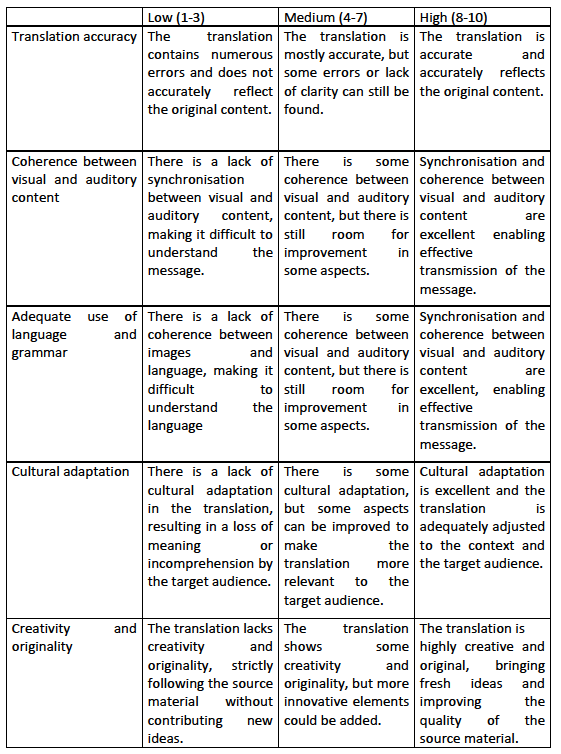
\includegraphics[width=\textwidth]{figure-annex.png}
  \caption{Assessment Rubrics.}
  \label{fig-annex}
  \source{Owm elaboration.}
\end{figure}

\section{Original Answers to the Questionnaire.}\label{annex-03}

Honelako ariketak egitea gustatuko litzaizuke? Zergatik?
\begin{enumerate}
  \item Bai, ikasiko nuelako.
  \item Bai, zeren asko gustatzen zait bideoak egitea.
  \item Bai, inoiz ez dudalako probatu eta ongi egongo zela uste dut.
  \item Bai, zeren asko gustatzen zait bideoak grabatzea.
  \item Bai, dibertigarria izango zelako.
  \item Ez, nahi dudalako Enara azaltzea.
  \item Ez.
\end{enumerate}


%conceptualization,datacuration,formalanalysis,funding,investigation,methodology,projadm,resources,software,supervision,validation,visualization,writing,review
\begin{contributors}[sec-contributors]
\authorcontribution{Edurne Goñi-alsúa}[conceptualization,methodology,review,resources,writing,visualization,supervision,projadm]
\authorcontribution{Galder Rejas Vicente}[formalanalysis,methodology,review,writing,investigation,datacuration,projadm]
\end{contributors}
\end{document}
